\documentclass[12pt]{article}

\usepackage{amsmath} % math
\usepackage{color} % support for color
\usepackage{hyperref} % turn citations into links
\usepackage[letterpaper,margin=1in,bottom=1in]{geometry} % margins
\usepackage{graphicx} % support for figures
\usepackage[numbers, sort & compress]{natbib} % cleanup citations
\usepackage{parskip} % add vertical space between paragraphs
\usepackage[section]{placeins} % keep figures inside their sections

\author{
  Pran Nath\footnote{Email: p.nath@northeastern.edu}~\ and
  Maksim Piskunov\footnote{Email: m.piskunov@northeastern.edu}\\~\\
  Department of Physics, Northeastern University,\\
  Boston, MA 02115-5000, USA
}

\title{
  Coherent Enhancement of the Decay Constant
  in Axionic Inflation in supersymmetry and strings
}

\begin{document}
\maketitle
\date

\textbf{Abstract:}
Models of axion inflation based on a single cosine potential require the axion decay constant to be super Planckian in size.
However, a super Plankian axion decay constant is disfavored in quantum gravity and in strings.
Here we propose a coherent enhancement mechanism which can produce an effective axion decay which is super Planckian even when the true axion decay constant is sub Planckian.
We discuss the utility of the coherent enhancement mechanism for a variety of axion potentials originating in supersymmetry, supergravity and strings.
The coherent enhancement mechanism allows one to reduce an inflation model with an arbitrary potential to an effective model of natural inflation, i.e. with a single cosine, by expanding the potential near an inflationary point, and matching the expansion coefficients to those of natural inflation.
We demonstrate that this approach can predict the number of e-foldings in a given inflation model without the need for numerical simulation.
Further we show that the effective decay constant $f_e$ can be directly related to the spectral indices so that $f_e = 1 / \sqrt{1 - n_s - r / 4}$ in Planck units where $n_s$ is the spectral index for curvature perturbations and $r$ is the ratio of the power spectrum of tensor perturbations and curvature perturbations.
Thus the current data on $n_s$ and $r$ constrains the effective axion decay constant so that $4.6 \leq f_e \leq 11$ at $95\%$ CL.
Thus an important result of the analysis is that the effective axion decay constant has an upper limit of $\sim 10$ in units of Planck mass in axion cosmology for any potential based model which produces successful inflation.
The coherent enhancement mechanism for the generation of an effective $f_e > 1$ while the true axion decay constant $f < 1$ is discussed.
We illustrate the coherent enhancement in several settings: globally supersymmetric models, supergravity models, in string setting including KKLT and Large Volume Scenario, and Dirac-Born-Infeld models.
In each case all the moduli are stabilized and the inflationary model consistent with astrophysical observations with $f_e > 1$ and the true axion decay constant $f < 1$ in Planck units.
\newpage

\section{Introduction \label{sec:Introduction}}
As is well known many of the problems associated with Big Bang cosmology which include
the flatness problem, the horizon problem, and the monopole problem are resolved by inflation~\cite{Guth:1980zm, Starobinsky:1980te, Linde:1981mu, Albrecht:1982wi, Sato, Linde:1983gd}.
Quantum fluctuations at the time of horizon exit carry significant information regarding specifics of the inflationary model~\cite{Mukhanov+, Cheung:2007st} which can be extracted from cosmic microwave background (CMB) radiation anisotropy.
The data from the Planck experiment~\cite{Adam:2015rua, Ade:2015lrj, Array:2015xqh} has helped constrain inflation models excluding some and narrowing down the parameter space of others.
One such model is so called natural inflation based on a $U(1)$ shift symmetry which is described by a simple potential~\cite{Freese:1990rb, Adams:1992bn} $V\left(a\right) = \Lambda^4 \left(1 - \cos(\frac{b}{f})\right)$, where $a$ is the axion field and $f$ is the axion decay constant.
In this case consistency with Planck data requires the axion decay constant to be significantly greater than the Planck mass $M_\text{P}$.
However, an axion decay constant larger than the Planck mass is undesirable since a global symmetry is not preserved by quantum gravity unless it has a gauge origin.
Additionally string theory prefers the axion decay constant to lie below $M_\text{P}$~\cite{Banks:2003sx, Svrcek:2006yi}.
It turns out that the reduction of the decay constant poses a problem, and several suggestions exist regarding its resolution such as the so called alignment mechanism~\cite{Kim:2004rp, Long:2014dta}.

A procedure for resolving the axion decay constant problem was proposed in~\cite{Nath:2017ihp}.
One element of this analysis relies on a decomposition of the potential into a fast-roll and a slow-roll parts where the slow roll is controlled only by the inflaton field while the remaining fields enter in fast roll and are not relevant for inflation~\cite{Nath:2017ihp} (for a review of inflation in supersymmetric theories see, e.g.,~\cite{Nath:2016qzm}).
An analysis within this model shows that one can obtain spectral indices as well as the ratio of the tensor to the scalar power spectrum consistent with the Planck data~\cite{Adam:2015rua, Ade:2015lrj, Array:2015xqh}.

The outline of the rest of the paper is as follows: In section \ref{sec:Alignment} we give a brief introduction to the alignment mechanism.
In section \ref{sec:CoherentEnhancement} we discuss the coherent enhancement mechanism when the potential consists of a superposition of cosines which is typically the case for axionic potentials we consider.
We exhibit the coherent enhancement in various settings.
Thus in section \ref{sec:Supersymmetry} we discuss this mechanism in globally supersymmetric models, in section \ref{sec:Supergravity} for supergravity models, in section \ref{sec:KKLT} for KKLT, in section \ref{sec:LVS} for the Large Volume Scenario, and in section \ref{sec:DBI} for the Dirac-Born-Infeld case.
Conclusions are given in section \ref{sec:Conclusion}.
Some relevant papers related to this work can be found in \cite{BlancoPillado:2006he, Conlon:2005jm, Ben-Dayan:2014lca, Gao:2014uha}.

\section{Alignment mechanism \label{sec:Alignment}}
An early work using QCD axions is the so-called natural inflation where the inflation potential is of the form
\begin{align} \label{eq:naturalInflationPotential}
  V(a) = \Lambda^4 \left(1 - \cos(\frac{\phi}{f})\right)\,,
\end{align}
$f$ is axion decay constant.
For a QCD axion $10^9 < f < 10^{12}$ GeV.
For inflation one requires $f > 10 M_\text{P}$.
However, $f > M_\text{P}$ is undesirable since global symmetry is not preserved by quantum gravity unless it has a gauge origin.
Further, string theory prefers $f$ in the range $\left(10^{16} - 10^{18}\right)$ GeV.
Thus to get a successful natural inflation is difficult.

One suggestion to realize $f < M_\text{P}$ is to use two axions and the alignment mechanism to achieve a flat direction.
For a model with two axions $\phi_1$ and $\phi_2$ one considers a potential
\begin{align} \label{eq:alignmentPotential}
  V(\phi) = \Lambda^4_1 \left[1 - \cos\left(\frac{\phi_1}{f_1} + \frac{\phi_2}{f_2}\right)\right]
          + \Lambda^4_2 \left[1 - \cos\left(\frac{\phi_1}{f_3} + \frac{\phi_2}{f_4}\right)\right]\,.
\end{align}
Constraint for a flat direction:
\begin{align}
  \frac{f_1}{f_2} = \frac{f_3}{f_4}\,.
\end{align}
However, the potential of Eq.~(\ref{eq:alignmentPotential}) appears it startes out by assuming that the same field has different decay constants, i.e., $\phi_1$ is associated with $f_1$ and $f_3$ and $\phi_2$ is associated with $f_2$ and $f_3$.
Here we discuss a new mechanism which can produce an effective decay constant that enters in inflation which is much larger than the true axion decay constant.

\section{General Analysis of Coherent Enhancement Mechanism \label{sec:CoherentEnhancement}}
Before we discuss the Coherent Enhancement Mechanism (CEM) we derive a relation what gives the effective axion decay constant directly in terms of the inflationary parameters and in terms of the experimentally measurable spectral indices.
Thus we consider a canonical Lagrangian of the form with a
\begin{equation}
  \mathcal{L}\left(\phi, \dot{\phi}\right) = \frac{1}{2}{\dot{\phi}}^2 - V\left(\phi\right)\,.
\end{equation}

Assuming the kinetic in canonically normalized in each case, it is sufficient to have $V\left(\phi\right) \approx V_{e}\left(\phi\right)$ where $V_{e}\left(\phi\right)$ is given by Eq.~(\ref{eq:naturalInflationPotential}) at $\phi \approx \phi_0$ to have similar evolution of the field and the scale factor near $\phi \sim \phi_0$.
Using this observation, we can express the parameters of natural Inflation $\Lambda$ and $f_e$ in terms of various order derivatives of $V\left(\phi\right)$.
To do that, first, expand $V_{e}$ near $\phi_0$ to the second order so that
\begin{equation} \label{eq:naturalInflationSeries}
  \begin{split}
    V_{e}\left(\phi\right) =
      &\Lambda \left(1 - \cos\left(\frac{\phi_0}{f_e}\right)\right)
        + \frac{\Lambda}{f_e} \sin\left(\frac{\phi_0}{f_e}\right) \left(\phi - \phi_0\right)\\
      & + \frac{\Lambda}{2 f_e^2} \cos\left(\frac{\phi_0}{f_e}\right) \left(\phi - \phi_0\right)^2
        + \mathcal{O}^3\left(\phi - \phi_0\right)\,.
  \end{split}
\end{equation}

Now, identifying the expansion coefficients in Eq.~(\ref{eq:naturalInflationSeries}) with corresponding derivatives of $V\left(\phi\right)$, and solving for $\Lambda$, $f_e$ and $\cos\left(\phi_0 / f_e\right)$, we obtain
\begin{equation} \label{eq:lambdaFromPotential}
  \Lambda = V\left(\phi_0\right) \frac
    {{V^\prime}^2\left(\phi_0\right) - V\left(\phi_0\right) V^{\prime\prime}\left(\phi_0\right)}
    {{V^\prime}^2\left(\phi_0\right) - 2 V\left(\phi_0\right) V^{\prime\prime}\left(\phi_0\right)}\,,
\end{equation}
\begin{equation} \label{eq:feFromPotential}
  f_e = \frac
    {V\left(\phi_0\right)}
    {\sqrt{{V^\prime}^2\left(\phi_0\right) - 2 V\left(\phi_0\right) V^{\prime\prime}\left(\phi_0\right)}}\,,
\end{equation}
\begin{equation} \label{eq:fieldInitialFromPotential}
  \cos\left(\frac{\varphi_0}{f_e}\right) = \frac
    {V\left(\phi_0\right) V^{\prime\prime}\left(\phi_0\right)}
    {{V^\prime}^2\left(\phi_0\right) - V\left(\phi_0\right) V^{\prime\prime}\left(\phi_0\right)}\,.
\end{equation}
Here, we are mostly interested in Eq.~(\ref{eq:feFromPotential}), which gives the effective axion decay constant for the potential $V\left(\phi\right)$ near $\phi = \phi_0$.
Due to second flatness condition, $\left|\eta_H\right| = \left|V_e^{\prime\prime} / V_e\right| = 1 / \left(2 f_e^2\right) \ll 1$, Natural Inflation can only generate experimentally consistent observables when $f_e \gg 1$.
However, as discussed already the true axion decay constant larger than one is undesirable from considerations of quantum gravity and string theory \cite{Kallosh:1995hi, Banks:2003sx}.
Coherent Enhancement provides a solution in that the true axion decay constants can be smaller than one while the effective axion decay constant is larger or even much larger than one.

Finally, it is also possible to express the effective decay constant in terms of slow-roll inflation parameters $\epsilon$ and $\eta$ defined as
\begin{equation} \label{eq:epsEtaFromPotential}
  \epsilon = \frac{1}{2} \left(\frac{V^\prime\left(\phi_0\right)}{V\left(\phi_0\right)}\right)^2\,,
  ~~~ \eta = \frac{V^{\prime\prime}\left(\phi_0\right)}{V\left(\phi_0\right)}\,.
\end{equation}

By combining these with Eqs.~(\ref{eq:lambdaFromPotential}, \ref{eq:feFromPotential}, \ref{eq:fieldInitialFromPotential}), we obtain
\begin{equation} \label{eq:lambdaSlowRoll}
  \Lambda = V\left(\phi_0\right) \frac{2 \epsilon - \eta}{2 \epsilon - 2 \eta}\,,
\end{equation}
\begin{equation} \label{eq:feSlowRoll}
  f_e = \frac{1}{\sqrt{2 \left(\epsilon - \eta\right)}}\,,
\end{equation}
\begin{equation} \label{eq:FieldInitialSlowRoll}
  \cos\left(\frac{\varphi_0}{f_e}\right) = \frac{\eta}{2 \epsilon - \eta}\,.
\end{equation}

The spectral indices $n_s$ and $n_t$ are related to the inflationary parameters so that
\begin{align} \label{eq:observablesSlowRoll}
  n_s = 1 - 6 \epsilon + 2 \eta\,,
  ~~~ n_t = -2 \epsilon\,,
  ~~~ r = 16 \epsilon\,.
\end{align}
We can thus eliminate $\eta$ and $\epsilon$ in favor of $n_s$ and $r$ and get
\begin{align}
  f_e = \frac{1}{\sqrt{1 - n_s - \frac{r}{4}}}\,.
\end{align}
The current experimental limits from Planck experiment at $k_0 = 0.05\,{\rm Mpc}^{-1}$ are as follows~\cite{Adam:2015rua, Ade:2015lrj, Array:2015xqh}
\begin{align} \label{data}
  n_s &= 0.9645 \pm 0.0049\, \left(68\%\, {\rm CL}\right)\,,\nonumber\\
    r &< 0.07\, \left(95\%\, {\rm CL}\right)\,,
\end{align}
while $n_t\left(k_0\right)$ is currently not constrained.
Using this data we find model independent bounds on the effective axionic decay constant so that
\begin{align}
  4.6 \leq f_e \leq 11\, \left(95\%\, {\rm CL}\right)\,.
\end{align}

Next we discuss CEM for a superposition of cosine functions and show how the effective axion decay constant becomes super-Planckian even though the true decay constant is sub-Plankian.
As a specific simple example let us consider a potential of the form
\begin{align} \label{eq:cosineSumPotential}
  V = \sum_{k = 1}^n \Lambda_k^4 \left(1 - \cos\left(\frac{k\phi}{f}\right)\right)\,.
\end{align}
Here let us choose $\phi_0$ where the maximum occurs so that $\frac{\phi}{f} = \pi$.
In this case we get
\begin{align} \label{eq:feForCosineSum}
  {f_e} / f = \frac
    {\sqrt{\sum_{k - odd} \Lambda_k}}
    {\sqrt{\left[\sum_{k - odd} k^2 \Lambda_k^4 - \sum_{k - even} k^2 \Lambda_k^4\right]}}\,.
\end{align}
Eq.~(\ref{eq:feForCosineSum}) holds in the limit when $\epsilon = 0$ which is, however, is typically small.
One notices that there is cancellation between the odd and even sums in the denominator in Eq.~(\ref{eq:feForCosineSum}) which leads to an enhancement and gives $f_e / f > 1$.
Since the enhancement occurs as a consequence of the sum of several terms one may call this a ``coherent enhancement mechanism''.

\section{Coherent enhancement mechanism in supersymmetry models \label{sec:Supersymmetry}}
In this section and the following sections we will discuss coherent enhancement mechanism in a variety of inflation models consistent with the current astrophysical data
from the Planck experiment. As mentioned in the introduction these models are in a variety of settings: global supersymmetry, supergravity,
KKLT, LVS and DBI. In this section we focus on the globally supersymmetric models.
For the analysis here we consider two chiral fields $\Phi_i, i=1,2$ charged under a global $U(1)$
transformation, and two other fields $\bar\Phi_i, i=1,2$ that are oppositely charged.
Thus under $U(1)$ transformations one
has
\begin{align}
  \Phi_i\to e^{i q \lambda} \Phi_i, ~~\bar \Phi_i\to e^{-i q \lambda} \bar \Phi_i, ~~i=1, \cdots, m\,.
\end{align}
The superfields ${\Phi}_{i}$ have an expansion,
${\Phi}_{i} = {\phi}_{i} + \theta {\chi}_{i} + \theta \theta {F}_{i}\,,$
where ${\phi}_{i}$ is a complex scalar field consisting of the saxion (the real part) and the axion (the imaginary
part), ${\chi}_{i}$ is the axino, and ${F}_{i}$ is an auxiliary field.
Similarly the superfields $\bar {\Phi}_{i}$ have an expansion:
$\bar {\Phi}_{i} = \bar {\phi}_{i} + \bar \theta \bar {\xi}_{i} + \bar\theta \bar \theta \bar{F}_{i}$.
We now consider a superpotential of the form
\begin{align}
  W = W_s(\Phi,\bar \Phi) + W_ {sb} (\Phi, \bar \Phi)\,,
  \label{wsn}
\end{align}
where $W_s$ is the part that depends on the fields $\Phi_i, \bar |phi_i$ and is invariant under the shift symmetry.
$W_{sb}$ is a part which breaks the shift symmetry. $W_s$ is chosen to stabilize the real parts of the chiral fields
and we expand the chiral fields around the stabilized VEVs. In this case we have
We may parametrize $\phi_i$ and $\bar \phi_i$ so that
\begin{align}
  \phi_i = (f_i + \rho_i) e^{ia_i/f_i}, ~~~\bar\phi_i = (\bar f_i + \bar \rho_i) e^{i\bar a_i/\bar f_i}\,,
\end{align}
where $f_i= <\phi_i> ,~\bar f_i= <\bar\phi_i>$ and $(\rho_i, a_i)$ and $(\bar \rho_i, \bar a_i)$
are the fluctuations of the quantum fields around their vacuum expectation values $f_i(\bar f_i)$.
We define two linear combinations of $a_1$ and $a_2$ so that
\begin{align}
  b_{\pm}= \frac{1}{\sqrt 2} (a_1\pm a_2)
  \label{b+b-}
\end{align}
Here $b_+$ is invariant under the shift symmetry and becomes heavy after the moduli are stabilized and $b_-$ is sensitive
to shift symmetry and remains massless and we identify it as a candidate for the inflaton. However, $b_-$ will gain mass
when $W_{sb}$ is included in the analysis. We will assume an $W_{sb}$ of the form
\begin{equation}
  W_{sb} \left( \Phi,\bar \Phi \right) =
  \sum_{i= 1}^{2} \sum_{l = 1}^{q} {A}_{i l} {\Phi}_{i}^{l} + \sum_{i = 1}^{2} \sum_{l = 1}^{q} {\bar{A}}_{i l} {\bar{\Phi}}_{i}^{l}\,.
  \label{wsn1}
\end{equation}
and violates the shift symmetry. Including $W_{sb}$ the axionic potential can be written in the form
\begin{align}
  V(a_1,a_2) = V_{\text{fast}}(b_+) + V_{\text{slow}}(b_-)
\end{align}
where $V_{\text{slow}}(b_-)$ which depends only on $b_-$ enters in slow roll and is relevant for inflation.
An explicit form of this potential is given by
\begin{align}
  {V}_{\text{slow}} (b_-) = & \sum_{k = 1}^{2} \Big[ 2 \sum_{r = 1}^{q} r \left( {A}_{k r} {f}^{r - 1} \sum_{l = 1}^{q} l {A}_{k l} {f}^{l - 1} + {\overline{A}}_{k r} {{f}}^{r - 1} \sum_{l = 1}^{q} l \overline{{A}}_{k l} {{f}}^{l - 1} \right) \times \nonumber\\
                            & \left( 1 - \text{cos} \left( \frac{r}{ \sqrt 2 f}
    {b}_{-}\right) \right)
    - 2 \sum_{l = 1}^{q} \sum_{r = l + 1}^{q} l r \left( {A}_{k l} {A}_{k r} {f}^{l + r - 2} + {\overline{A}}_{k l} {\overline{A}}_{k r} {{f}}^{l + r - 2} \right)\nonumber\\
                            & \times \left( 1 - \text{cos} \left( \frac{r - l}{\sqrt 2 f } {b}_{-}\right) \right) \Big]\,.
  \label{slow1}
\end{align}
where we have set $\bar f_k=f_k=f$ for all $k$.
We make now further simplifying assumptions so that
${A}_{k l} = {\overline{A}}_{k l} = {B}_{l} {f}^{3 - l}$, ${B}_{l} = B {G}_{l}$, ${f}_{k} = f$ for all $k$. Thus $B_l, B, G_l$ are dimensionless while $f_k=f$ carry dimension of mass. Using the above assumptions
e the potential of Eq.(\ref{slow1}) takes the form simpler form
\begin{equation}
  \begin{aligned}
    {V}_{\text{slow}} \left( {b}_{-} \right) =
    4 m {f}^{4} {B}^{2} \Big( \sum_{l = 1}^{q} l {G}_{l} \sum_{r = 4}^{q} r {G}_{r} \left( 1 - \text{cos} \left( \frac{r}{\sqrt{2 m}} \frac{{b}_{-}}{f} \right) \right) \\
    - \sum_{l = 1}^{q} \sum_{r = l + 4}^{q} l r {G}_{l} {G}_{r} \left( 1 - \text{cos} \left( \frac{r - l}{\sqrt{2 m}} \frac{{b}_{-}}{f} \right) \right) \Big)\,.
    \label{slow2}
  \end{aligned}
\end{equation}
Eq.(\ref{slow2}) will be used in our computations.\\

% TODO(maxitg): Simulation part needs to be added here.

\section{\bf Enhancement mechanism in supergravity \label{sec:Supergravity}}
We now extend the analysis to supergravity where the scalar potential has the form~\cite{Chamseddine:1982jx,Cremmer:1982en}
is given by
\begin{align}
  V= e^K [ D_i W K^{-1}_{ij^*} D_{j^*} W^* - 3 |W|^2] + V_D\,,
  \label{sugra1}
\end{align}
where $K$ is the K\"ahler potential, $W$ as before is the superpotential $D_iW$ is defined by

\begin{align}
  D_i W= \frac{\partial W}{\partial \phi_i} + \frac{\partial K}{\partial \phi_i} W\,.
  \label{sugra2}
\end{align}
$V_D$, which is the $D$-term of the potential will play no role in our analysis and will we dropped from here on.
In order to avoid the so-called $\eta$ -problem of supergravity we choose the K\"ahler potential to be of the form
\begin{align}
  K = \sum_{i} \frac{1}{2} (\Phi_i+ \Phi_i^\dagger)^2\,,
\end{align}
where as in the global supersymmetry model we consider a pair of chiral fields $\Phi_i$ (i=1,2).
We parametrize the complex scalar component of the fields so that
$\phi_i$ of $\Phi_i, i=1,2$ so that
\begin{align}
  \phi_i = (\rho_i + i a_i)/\sqrt 2,~ i=1,2\,,
\end{align}
where $ a_i$ have the shift property
\begin{align}
  a_1\to a_1 + \lambda, ~~a_2\to a_2 - \lambda\,,
\end{align}
and $\rho_i$ are the saxion fields. It is then easily checked the the kinetic energy for $\phi_i$ and $a_i$ are
canonically normalized.
As in the global supersymmetry case we choose $W$ of the form Eq.(\ref{wsn})  where, however, we write
\begin{align}
  W_s = W_s^{\text{vis})} + W_0
\end{align}
Where $W_s$ is invariant under the shift symmetry with $W_s^{\text{vis})}$ asking from the visible sector
and $W_0$ arising from the hidden sector. For supergravity analysis the saxion can be stabilized by imposition of spontaneous symmetry breaking
conditions~\cite{Nath:1983aw}
\begin{align}
  D_iW =0, i=1,2
\end{align}
For shift symmetry breaking we assume
\begin{align}
  W_{sb} = \sum_{n=1}^q A_n \left ( e^{c_n\Phi_1} + e^{c_n\Phi_2}\right)\,.
\end{align}
and as in the global supersymmetry case we make a change of basis from $a_1, a_2$ to $b_+, b_-$ as given by
Eq.(\ref{b+b-}).
Next we expand around the minimum of the saxion potential and retain only $b_-$ which controls the
the slow roll part of the potential. To that end
$W_{sb}$ takes the form
\begin{align}
  W_{sb}= -\sum_{n=1}^q B_n (e^{i\gamma_n\frac{b}{\sqrt 2 f}} + e^{-i\gamma_n \frac{b}{\sqrt 2f}})\,.
\end{align}
where $B_n= - A_n e^{c_n f/\sqrt 2}$ and $\gamma_n = c_n f/\sqrt 2$.
in addition to the stabilization of the saxions we also impose vanishing of the vacuum energy
at the end of inflation. In this case the slow roll part of the potential which involves only the field $b_-$ takes the form

\begin{align}
  V(b_-) & =
  e^{2f^2}\Big[
    2\sum_{n=1}^q\sum_{m=1}^q c_nc_mB_nB_m \left(1- 2 \cos(\frac{\gamma_n b_-}{\sqrt 2 f}) + \cos((\gamma_n-\gamma_m) \frac{b}{\sqrt 2 f})\right)\nonumber\\
         & + \sum_{n=1}^q\sum_{m=1}^q
    (16 f^2 + 8 \sqrt 2 f c_n -12)B_nB_m
    \Big(1- \cos(\gamma_n b_-/ \sqrt 2f)- \cos(\gamma_m b_-/ \sqrt 2f) \nonumber\\
         & +\frac{1}{2} \cos((\gamma_n-\gamma_m) b_-/ \sqrt 2f)+ \frac{1}{2} \cos((\gamma_n+\gamma_m) b_-/ \sqrt 2f)
    \Big)
    \Big]\,.
  \label{sugrapot}
\end{align}
The above potential consists of a superposition of six cosines so that

\begin{align}
  V(b_-)= \sum_{k=1}^{6} C_k \left(1-\cos(\frac{kb_-}{\sqrt 2 f})\right)
\end{align}
where $C_k$ are given by

\begin{align}
  C_1 = & - \frac{1}{f^2} (4 {e}^{2 {f}^{2} + 2} ( - 2 {A}_{1}^{2} \left( 4 {f}^{4} + {f}^{2} + 1 \right) - e {A}_{1} \left( {A}_{2} \left( 4 {f}^{2} + 3 \right)  {f}^{2} + 2 e {A}_{3} \left( 4 {f}^{4} + 5 {f}^{2} + 3 \right) \right) \nonumber\\
        & + {e}^{3} {A}_{2} {A}_{3} \left( 4 {f}^{4} + 7 {f}^{2} + 12 \right) ))\nonumber\\
  C_2= & + \frac{1}{f^2}(2 {e}^{2 {f}^{2} + 2} ( {A}_{1}^{2} \left( - \left( 4 {f}^{4} + {f}^{2} \right) \right) + 2 e {A}_{1} \left( {A}_{2} \left( 8 {f}^{4} + 6 {f}^{2} + 4 \right) - e {A}_{3} \left( 4 {f}^{4} + 5 {f}^{2} + 6 \right) \right) \nonumber\\
        & + 4 {e}^{2} {A}_{2} \left( {A}_{2} \left( 4 {f}^{4} + 5 {f}^{2} + 4 \right) + e {A}_{3} \left( 4 {f}^{4} + 7 {f}^{2} + 6 \right) \right) ))\nonumber\\
  C_3= & + \frac{1}{f^2}(4 {e}^{2 {f}^{2} + 3} ( {A}_{1} \left( 2 e {A}_{3} \left( 4 {f}^{4} + 5 {f}^{2} + 3 \right) - {A}_{2} {f}^{2} \left( 4 {f}^{2} + 3 \right) \right) \nonumber\\
        & + 2 {e}^{2} {A}_{3} \left( {A}_{2} \left( 4 {f}^{4} + 7 {f}^{2} + 6 \right) + e {A}_{3} \left( 4 {f}^{4} + 9 {f}^{2} + 9 \right) \right) ))\nonumber\\
  C_4= & - 2 \left( {A}_{2}^{2} + 2 {A}_{1} {A}_{3} \right)  {e}^{2 {f}^{2} + 4} \left( 4 {f}^{2} + 5 \right) \nonumber\\
  C_5= & - 4 {A}_{2} {A}_{3} {e}^{2 {f}^{2} + 5} \left( 4 {f}^{2} + 7 \right) \nonumber\\
  C_6= & - 2 {A}_{3}^{2} {e}^{2 {f}^{2} + 6} \left( 4 {f}^{2} + 9 \right)
  \label{c1}
\end{align}

% TODO(maxitg): Simulation part needs to be added here.

\section{Coherent axion enhancement in KKLT\label{sec:KKLT}}
We wish to discuss coherent enhancement of the decay constant in KKLT~\cite{Kachru:2003aw}.
The scalar potential of the theory is as given by Eq.(\ref{sugra1}) and Eq.(\ref{sugra2}).
In the KKLT analysis we consider a K\"ahler potential with a single modulus $T$ so that

\begin{align}
  K = -3 \, \text{log}(T+ \bar T)\,,
  \label{kklt1}
\end{align}
where we may decompose $T$ so that
$T= \tau + i \theta$.
We assume the superpotential $W$ where the modulus dependence arises only in the anon-perturbative terms
and we take $W$ to have the form
\begin{align}
  W= W_0 +\sum_{i} A_i e^{- q_iT}\,,
  \label{w0A}
\end{align}
where the modulus $T$ appears only in the exponent and where $A_i$ and $q_i$ are assumed real.
For the K\"ahler potential of Eq.(\ref{kklt1}) the scalar potential Eq. (\ref{sugra1}) takes the form

\begin{align}
  V= e^K K^{T\bar T} \left[\partial_TW \partial_{\bar T} \bar W +
    (\partial_TK W \partial_{\bar T} \bar W +
    \partial_{\bar T} K \bar W \partial_{T} W) \right]\,.
\end{align}
An explicit computation of $V$ gives
\begin{align}
  V= & \frac{1}{6\tau} \Big [ \sum_{i} A^2_i q^2_i e^{- 2q_i \tau } + 2 \sum_{i>j} A_iA_j q_iq_j e^{-(q_i+q_j)\tau} \cos\left((q_i-q_j) \theta\right)\nonumber\\
     & + \frac{3}{\tau} W_0 \sum_i A_i q_i e^{-q_i \tau} \cos(q_i \theta)
    + \frac{3}{\tau} \
    \sum_{i,j} A_i A_j q_j e^{-(q_i + q_j) \tau} \cos((q_i -q_j)\theta)
    \Big]
  \label{11}
\end{align}
To stabilize the modulus $\tau$ we use the condition~\cite{Nath:1983aw}
\begin{align}
  D_{,T} W =0
  \label{33.1}
\end{align}
which gives the constraint
\begin{equation}\label{eqn:crit}
  W_0 = -\sum_i A_i e^{-q_i\tau_0} \left(1 + \frac{2}{3} q_i \tau_0\right)\, ,
\end{equation}
where $<T>=\tau_0, <\theta>=0$.
Next wer expand $T$ around the critical point, i.e.,
$T= \tau_0 + \tau' + \theta$. However, the kinetic energy using $\tau$ and $\theta$ is not canonically normalized
and we define the normalized fields $\rho, a$ so that
\begin{align}
  \rho \equiv \frac{\sqrt 3}{\sqrt 2 \tau_0} \tau',~ a \equiv \frac{\sqrt 3}{\sqrt 2 \tau_0}\theta\,,
  \label{19}
\end{align}
for which the kinetic energy takes the canonical form, i.e,
$L_{kin}=
  - \frac{1}{2}
  \left[\partial_\mu \rho \partial^\mu \rho + \partial_\mu a \partial^\mu a\right]\,.$ Using the canonically normalized fields
we can define the axion decay constant so that $f= \frac{\sqrt 3}{\sqrt 2 \tau_0}$.
The potential for the normalized axion field expanded around the stabilized moduli gives
\begin{align}
  V(a)= & \frac{1}{6\tau_0} \Big [ \sum_{i} A^2_i q^2_i e^{- 2q_i \tau_0 } + 2 \sum_{i>j} A_iA_j q_iq_j e^{-(q_i+q_j)\tau_0}
    \cos\left(\frac{(q_i-q_j) a}{f}\right)\nonumber\\
        & + \frac{3}{\tau_0} W_0 \sum_i A_i q_i e^{-q_i \tau_0} \cos(\frac{q_i a}{f})
    + \frac{3}{\tau_0} \
    \sum_{i,j} A_i A_j q_j e^{-(q_i + q_j) \tau_0} \cos\left(\frac{(q_i -q_j)a}{f}\right)
    \Big]
  \label{24}
\end{align}
We require that the vacuum energy vanish at the minimum of the potential, and this can be achieved by setting $W=0$ along with the
stability condition $D_i W =0$. These conditions lead to the constraint

\begin{align}
  \sum_i A_i q_i e^{-q_i \tau_0}=0
  \label{27}
\end{align}
The imposition of Eqs. (\ref{33.1}) and (\ref{27}) would lead to moduli stabilization and
vanishing of the vacuum energy at the end of inflation. \\

% TODO(maxitg): Simulation part needs to be added here.

\section{Inflation in Large Volume Scenario (LVS) \label{sec:LVS}}

Next we consider the Large Volume Scenario (LVS) \cite{Balasubramanian:2005zx}
where the K\"ahler potential has the form

\begin{equation}
  K = - \, \text{log} (S+ \bar{S}) -2 \, \text{log} (\mathcal{V} +\alpha)
  + K_{cs} (U, \bar{U})  \, ,
\end{equation}
Here $S$ is the dilation, $U$ are the complex moduli. For moduli stabilization we need $\alpha$-correction to the K\"ahler potential where
and $\alpha = \frac{1}{2} \xi S_1^{3/2}$ where $\xi = -\zeta (3) \chi/2 (2\pi)^3$, and $\chi$ is the topological Euler characteristic of $X$ of the compact manifold. For $\mathcal{V}$ we consider a Kahler moduli space
with $h^{1,1}(X)=2$ and in this case one may write $\mathcal{V}$ in the form
\begin{equation}
  \mathcal{V} = \eta \,( \tau_b^{3/2} - \tau_s^{3/2}) \, .
\end{equation}
In the analysis we will assume that $S$ and $U$ have been stabilized at large scales and thus these will play no role in the
inflation analysis. We will thus focus on the stabilization of the remaining moduli. Here we assume a superpotential of the form

\begin{align}
  W= W_0 +\sum_i A_i e^{-q^i_b \tau_b -q^i_s \tau_s}
\end{align}
The computation of the $V$ in this case gives


\begin{align}
  V= & \frac{2 W_0}{S_1 \mathcal{V}^2} \sum_i (\tau_b q_b^i +\tau_s q_s^i) A_i e^{- q_b^i \tau_b - q_s^i \tau_s} \cos(q_b^i \theta_s + q^i_s \theta_s) \nonumber\\
     & + \frac{1}{3 S_1\mathcal{V}^2} \sum_{i,j} \Big[3 \tau_b (q^i_b +q^j_b)
    + 3\tau_s (q_s^i +q_s^j)
    + 2 (\tau_b^2 + 2 \sqrt \tau_b \tau_s^{3/2}) q_b^i q_b^j \nonumber\\
     & + 2(\tau^2_s+2 \sqrt{\tau_s} \tau^{3/2}_b) q_s^i q_s^j + 6 \tau_b \tau_s (q_b^i q_s^j + q_b^j q_s^i) \big]\nonumber\\
     & \times
  A_i A_j e^{ -(q_b^i + q_b^j) \tau_b - (q_s^i + q_s^j)\tau_s} \cos\left((q_b^i -q_b^j)\theta_b + (q_s^i -q_s^j)\theta_s\right) + \Delta V
\end{align}
where $\Delta V$ contains $\alpha'$ corrections. Next to stabilize the moduli we use the condition
\begin{align}
  D_i W==0, i= \tau_b, \tau_s, \theta_b, \theta_s\,.
\end{align}
The stabilization leads to $<\theta_b>=<\theta_s>=0$, $<\tau_b>=\tau_{b0}$ and $<\tau_{s}>= \tau_{s0}$ where
$\tau_{s_0}$ and $\tau_{b0}$ are constrained by

\begin{align}
  \sum_i q^i_b A_i e^{-q_b^i \tau_{b0} - q^i_s \tau_{s0}} +
  \frac{3 \sqrt {\tau_{b0}}}{2 (\tau^{3/2}_{b0}- \tau^{3/2}_{s0})} \left( W_0 + \sum_i A_i e^{-q^i_b \tau_{b0} - q_s^i \tau_{s0}} \right) =0.
  \label{lvs-stabiltiy-1}
\end{align}
Further, for vanishing of the vacuum energy at the end of inflation we impose the constraint $<W>=0$ which gives
\begin{align}
  W_0 + \sum_i A_i e^{- q_b^i \tau_{b0} - q_s^i \tau_{s0}} =0.
\end{align}
For $\Delta V$, which is needed to achieve stability,
we choose the conventional LVS correction to the potential, i.e.,
\begin{align}
  \Delta V= \xi \frac{3 |W_0|^2 \sqrt {S_1}}{8 \mathcal{V}^3}
\end{align}
% TODO(maxitg): Simulation part needs to be added here.

\section{Coherent Enhancement Mechanism for Dirac-Born-Infeld \label{sec:DBI}}
Supersymmetric DBI actions have been investigated by a number of authors
(see, e.g., \cite{Khoury:2010gb,Khoury:2011da,Baumann:2011nk,Baumann:2011nm,Rocek:1997hi,Tseytlin:1999dj,Ito:2007hy,Billo:2008sp,Sasaki:2012ka,Aoki:2016tod}.
Here we discuss the supersymmetric DBI in the context of axion inflation.
Inflation in a single field DBI has discussed in \cite{Sasaki:2012ka} and for the case of two fields in~\cite{Nath:2018xxe}.
Here we discuss the coherent enhancement mechanism in the context of the two fields.
Thus as in our analysis in sections 4 and 5 we consider a pair of chiral superfields $\Phi_1$ and $\Phi_2$ which carry opposite
charges under a global $U(1)$ symmetry.
The supersymmetric Lagrangian involving $\Phi_1$ and $\Phi_2$ is given by
\begin{equation}
  \mathcal{L}= \mathcal{L}_D+\mathcal{L}_{F},
  \label{1.1}
\end{equation}
where $\mathcal{L}_D$ is the D-part of the Lagrangian and $\mathcal{L}_{F}$ is the F-part. Here $\mathcal{L}_D$
consists of a part which is quadratic in the fields and a part which is quartic in the fields so that
\begin{align}
  \mathcal{L}_D
   & = \int d^4\theta \left(\Phi_1 \Phi_1^\dagger + \Phi_2 \Phi_2^\dagger \right)+ \int d^4\theta
  \frac{\alpha_1}{16T}\left(D^\alpha \Phi_1 D_\alpha \Phi_1\right)\left({\bar{D}}^{\dot{\alpha}}\Phi_1^\dagger {\bar{D}}_{\dot{\alpha}}\Phi_1^\dagger \right)
  G(\phi),
  \label{Lag.11}
\end{align}
where
\begin{align}
  G(\phi) = \frac{1}{T}\frac{1}{1+ P +\sqrt{(1+P)^2 -Q}},
\end{align}
and $P$ and $Q$ are assumed to have the following forms
\begin{align}
  P & = (\partial_a\phi_1 \partial^a \phi^*_1 + \partial_a\phi_2 \partial^a \phi^*_2)/T, \nonumber\\
  Q & = \Big(
  \alpha_1\partial_a \phi_1 \partial^a \phi_1 \partial_b \phi^*_1 \partial^b \phi^*_1
  + \alpha_1 \partial_a \phi_2 \partial^a \phi_2 \partial_b \phi^*_2 \partial^b \phi^*_2
  \Big) / T^2.
  \label{Lag.22}
\end{align}
We note that the Lagrangian of Eq.~(\ref{Lag.11}) is a direct generalization of the Lagrangian for the single field
case which can be derived from a more basic 3-brane action
(see, e.g., \cite{Rocek:1997hi,Tseytlin:1999dj,Sasaki:2012ka} and the references
therein). Here we simply extend the analysis to two fields
in the most general supersymmetric form involving four covariant derivatives. In writing Eq.~(\ref{Lag.11}) we imposed
an additional constraint which is invariance under $\Phi_1$ and $\Phi_2$ interchange.
The possible relation of this Lagrangian
to an underlying string model is an open question. Here we simply treat Eq.~(\ref{Lag.11}) as an effective low energy
theory. Finally $\mathcal{L}_{F}$ is given by
\begin{equation}
  \mathcal{L}_{F}=\int d^2\theta W\left(\Phi_1,\Phi_2\right)+\int d^2\bar\theta
  W^* \left(\Phi_1^\dagger,\Phi_2^\dagger\right),
\end{equation}
where the superpotential $W$ as in earlier analyses is given by $W=W_s+W_{sb}$, and where
$W_s$ is chosen so that we can stabilize the saxion VEVs
and $W_{sb}$ breaks the global $U(1)$ symmetry and is taken to be of the form
\begin{equation}
  W_{sb}=\sum_{k=1}^m\left(A_{1, k}\Phi_1^k+A_{2, k}\Phi_2^k\right).
  \label{w3}
\end{equation}
Integration over the Grassmann variables gives rise to the following Lagranian\\
\begin{align}
  \mathcal{L}
   & =
  T - T \sqrt{(1+A)^2 - B}+ F_1 F^*_1 + F_2 F^*_2\nonumber\\
   & + G(\phi) \Big[ \alpha_1(-2 F_1 F^*_1 \partial_a\phi_1 \partial^a \phi^*_1
    + F_1^2 {F^*_1}^2)\nonumber\\
   & + \alpha_1 (-2 F_2 F^*_2 \partial_a\phi_2 \partial^a \phi^*_2
    + F_2^2 {F^*_2}^2)\Big]
  \nonumber\\
   & + \left(\frac{\partial W}{\partial \phi_1}F_1+ \frac{\partial W}{\partial \phi_2}F_2 + h.c.\right).
  \label{Lag.23}
\end{align}
There are four auxiliary fields in Eq.~(\ref{Lag.23}) which are $F_1, F^*_1, F_2, F^*_2$.
The auxiliary fields $F_k$ satisfy the cubic equation
\begin{align}
  F_k^3+ p_k F_k + q_k=0\,, k=1,2\,,
\end{align}
where $p_k, q_k$ are defined by
\begin{equation}\label{DisplayFormulaNumbered:eq.twoDBI.p.1}
  \begin{split}
    & p_k={\left(\frac{\partial W}{\partial \phi_k}\right)}^{-1}\frac{\partial W^*}{\partial \phi^*_k}\frac{1-2\alpha_1 G\left(\phi\right)\partial_\mu \phi_k\partial^\mu \phi_k}{2\alpha_1 G\left(\phi\right)}, \\
    & q_k=\frac{1}{2\alpha_1 G\left(\phi\right)}{\left(\frac{\partial W}{\partial \phi_k}\right)}^{-1}{\left(\frac{\partial W^*}{\partial \phi^*_k}\right)}^2. \\
  \end{split}
\end{equation}
Since $F_k$ satisfies a cubic equation, it has three roots which are
\begin{equation}
  \begin{split}
    F_k=& \omega^j {\left(-\frac{q_k}{2}+\sqrt{ {\left(\frac{q_k}{2}\right)}^2+{\left(\frac{p_k}{3}\right)}^3}\right)}^{1/3}\\
    &+ \omega^{3-j}{\left(-\frac{q_k}{2}-\sqrt{ {\left(\frac{q_k}{2}\right)}^2+{\left(\frac{p_k}{3}\right)}^3}\right)}^{1/3},
  \end{split}
  \label{auxsolution}
\end{equation}
where $\omega$ is the cube root of unity and $j=0,1,2$. It turns out that of the three roots only $j=0$
is a solution to the full Euler-Lagrange equations for $F_k$ and in our analysis we consider only this solution.

An explicit computation of the Lagrangian in this case is given in \cite{Nath:2018xxe} and displayed in Eq.(\ref{DisplayFormulaNumbered:eq.dbi.lagrangian}).
The Lagrangian depends on a single axion field $b_-$ defined as in the preceding sections
and 5 parameters $T$, $\alpha_1$, $f$, $\tilde \beta$, and a vector $\mathcal{G}$ as discussed below.
Thus we have
\begin{equation}\label{DisplayFormulaNumbered:eq.dbi.lagrangian}
  \begin{split}
    & \mathcal{L}\left(T,\alpha_1,f,\beta,G;b_-,\dot{b_-}\right)=T \left(1-\sqrt{1-\frac{{\dot{b}}_-^2}{T}+\frac{\left(2-\alpha_1\right){\dot{b}}_-^2}{8T^2}}\right. \\
    & \indent\indent\left.{}+2\mathcal{F}_+^2+2\mathcal{F}_-^2-\frac{4}{3\alpha_1}\left(\mathcal{T}+\left(\alpha_1-1\right)\frac{{\dot{b}}_-^2}{4T}\right)+4k \left(\mathcal{F}_++\mathcal{F}_-\right)\right. \\
    & \indent\indent\left.{}+\frac{\alpha_1}{\mathcal{T}-{\dot{b}}_-^2/\left(4T\right)}\left(2\left(\mathcal{F}_+^2+\mathcal{F}_-^2-\frac{2}{3\alpha_1}\left(\mathcal{T}+\left(\alpha_1-1\right)\frac{{\dot{b}}_-^2}{4T}\right)\right)\frac{{\dot{b}}_-^2}{4T}+\mathcal{F}_+^4\right.\right. \\
    & \indent\indent\indent\left.\left.{}+\mathcal{F}_-^4+\frac{2}{3\alpha_1^2}{\left(\mathcal{T}+\left(\alpha_1-1\right)\frac{{\dot{b}}_-^2}{4T}\right)}^2-\frac{4}{3\alpha_1}\left(\mathcal{T}+\left(\alpha_1-1\right)\frac{{\dot{b}}_-^2}{4T}\right)\left(\mathcal{F}_+^2+\mathcal{F}_-^2\right)\right)\right),
  \end{split}
\end{equation}
where
\begin{equation}
  \begin{split}
    & \mathcal{F}_\pm=\pm\left(\mp\frac{1}{2\alpha_1}k \left(\mathcal{T}-\frac{{\dot{b}}_{-}^2}{4T}\right)\right. \\
    & \indent\indent\left.{}+\sqrt{ \frac{1}{4\alpha_1^2} k^2 {\left(\mathcal{T}-\frac{{\dot{b}}_{-}^2}{4T}\right)}^2+\frac{1}{27\alpha_1^3}{\left(\mathcal{T}+\left(\alpha_1-1\right)\frac{{\dot{b}}_{-}^2}{4T}\right)}^3}\right)\mathit{p}^{1/3},
  \end{split}
\end{equation}
and where

\begin{equation}
  \mathcal{T}=\frac{1}{2} \left(1+\sqrt{1-\frac{{\dot{b}}_-^2}{T}+\frac{\left(2-\alpha_1\right){\dot{b}}_-^4}{8T^2}}\right),
\end{equation}

\begin{equation}
  \begin{split}
    & k=\tilde\beta\sqrt{\sum_{m, n}m n \mathcal{G}_m\mathcal{G}_n \left(1-\cos\left(\frac{b_- m}{\sqrt{2}f}\right)-\cos\left(\frac{b_- n}{\sqrt{2}f}\right)+\cos\left(\frac{b_- \left(m-n\right)}{\sqrt{2}f}\right)\right)},
  \end{split}
\end{equation}
\begin{equation}
  \mathcal{G}_k=\frac{A_k2^{1/2\left(1-k\right)}}{\tilde\beta\sqrt{T}f^{1-k}}.
\end{equation}


We note that the parameter $\tilde\beta$ here is redundant, and is chosen in such a way as to make $\mathcal{G}_k\sim 1$. The first non-zero component of $\mathcal{G}$ can also be set to $1$ to reduce redundancy.
Further, we note that Eqs.(\ref{DisplayFormulaNumbered:eq.epsilonV}) will not be sufficient to describe evolution in this case, because they do not take the form of kinetic energy into account. However, we will use
Eqs.(\ref{DisplayFormulaNumbered:eq.epsilon}) which are independent of the kinetic terms, therefore, we conjecture that while Eqs.(\ref{DisplayFormulaNumbered:eq.epsilon.fromEpsilonEtaV}) do not hold, Eq.(\ref{DisplayFormulaNumbered:eq.fe.epsilonEta}) can still be used to derive an effective decay constant, where Eqs.(\ref{DisplayFormulaNumbered:eq.epsilon}) are used to derive $\epsilon_H$ and $\eta_H$.

\begin{equation}\label{DisplayFormulaNumbered:eq.epsilon}
  \epsilon_H =-\frac{\dot{H}}{H^2}\,,
  ~~\eta_H =-\frac{\dot{\epsilon_H}}{\epsilon_H H},
\end{equation}
For the case when the velocity dependence of the parameters is relatively small one has
\begin{equation}\label{DisplayFormulaNumbered:eq.epsilon.fromEpsilonEtaV}
  \epsilon_H =\epsilon\,,
  ~~\eta_H =-2\eta+4\epsilon,
\end{equation}
in which case Eqs.(\ref{DisplayFormulaNumbered:eq.lambda.slowRoll}, \ref{DisplayFormulaNumbered:eq.fe.slowRoll}, \ref{DisplayFormulaNumbered:eq.fieldInitial.slowRoll}) can be rewritten as

\begin{equation}
  \Lambda =V\left(\phi_0\right)\frac{\eta_H}{2\eta_H -4\epsilon_H},
\end{equation}

\begin{equation}\label{DisplayFormulaNumbered:eq.fe.epsilonEta}
  f_e=\frac{1}{\sqrt{\eta_H -2\epsilon_H}}.
\end{equation}

\begin{equation}
  \cos\left(\frac{\varphi_0}{f_e}\right)=\frac{4\epsilon_H -\eta_H}{\eta_H}.
\end{equation}

To demonstrate the validity of our procedure, we sample the parameter space of the model Eq.(\ref{DisplayFormulaNumbered:eq.dbi.lagrangian}) by setting $T=1$, $\mathcal{G}_1=\mathcal{G}_2=\mathcal{G}_3=0$, $\mathcal{G}_4=1$, and varying $\mathcal{G}_5$, $\mathcal{G}_6$, $\alpha_1$, $f$, $\tilde\beta$, and the pivot e-foldings count $N_{pivot}$. This corresponds to Fig.(1) of \cite{Nath:2018xxe}. We then select parameter choices than produced at least $N_{pivot}$ number of e-foldings, and plot the true axion decay constant $f$ vs. the effective axion decay constant $f_e$ on Fig.(\ref{Figure:fig.enhancement.sim}).\\

% TODO(maxitg): Simulation part needs to be added here.

\section{Conclusion \label{sec:Conclusion}}
One of the possible candidates for inflation is an axion. However, axion models with a simple cosine potential
require an axion decay constant which is super Planckian in size which is not favored in quantum gravity and strings.
One early proposal to overcome this problem is the so called alignment mechanism where one considers two or more
axion fields and imposes certain constraints on the decay constants. Here we propose a new mechanism, the coherent
enhancement mechanism, which allows one to produce an effective decay constant which governs inflation to be much
larger than the true decay constant. The mechanism is quite general and applies naturally to axion potential arising
in models based in supersymmetry, supergravity and strings. We illustrated the mechanism for supersymmetric
models and for KKLT and LVS type models. A brief analysis for the case of DBI was also discussed.
One of the interesting results of the analysis is that the effective decay constant can be directly related to the spectral indices.

\textbf{Acknowledgments:}
This research was supported in part by the NSF Grant PHY-1620575.

\clearpage

\begin{figure}
  \centering
  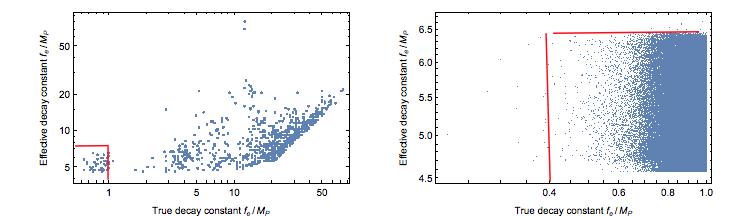
\includegraphics[width=0.8\textwidth]{figs/figsusy.png}
  \caption{ Comparison of true vs. enhanced axion decay constants for model Eq.(13) with $G_6 = 0$ (left panel) and
    $G_6 \neq 0$ (right panel). Data corresponds to Figs. (3, 5) of \cite{Nath:2017ihp}.
    The number of points is 939 on the left, and 102492 on the right panel.
    Note that while there are points with true decay constants below
    MP, all of the enhanced decay constants are larger than $4.5 M_P$, which is
    necessary for produce a sufficient number of e-foldings in Natural Inflation.}
  \label{figsusy}
\end{figure}

\begin{figure}
  \centering
  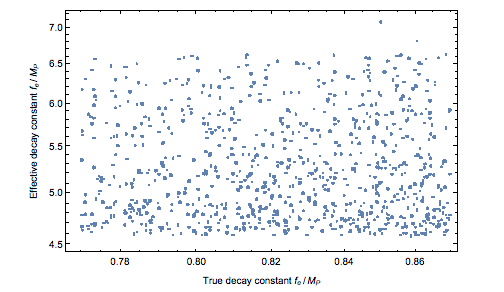
\includegraphics[width=0.8\textwidth]{figs/figsugra.png}
  \caption{ Comparison of true vs. enhanced axion decay constants for model Eq. (\ref{c1}). Data corresponds to Figs.(9, 10) of [7]. The number of points is 846. Note that while all true decay constants are smaller than $M_P$, all enhanced decay constants are larger than
    $4.5 M_P$, which is necessary for produce the number of e-foldings in the desired range.}
  \label{figsugra}
\end{figure}

\begin{figure}
  \centering
  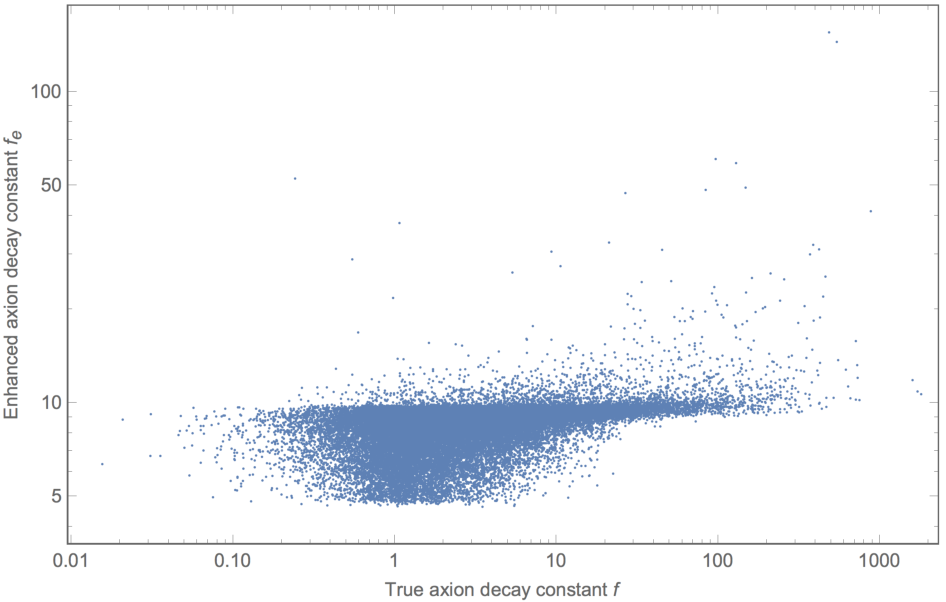
\includegraphics[width=0.5\textwidth]{figs/fige.pdf}
  \caption{Comparison of true vs. enhanced axion decay constants for model Eq.(\ref{DisplayFormulaNumbered:eq.dbi.lagrangian}), $33418$ points shown ($13$ points for which $\eta - 2\epsilon < 0$ are excluded from analysis). Note that while the true decay constants vary from $\sim 0.01$ to $\sim 2000$, all of the enhanced decay constants are larger than $4.6$, and have an average of $8.4$. Note further than the minimal value of ${f}_{e}$ in Natural Inflation required to produce experimentally consistent inflation is ${f}_{e} \approx 6.9$ \cite{Ade:2015lrj}.}
  \label{Figure:fig.enhancement.sim}
\end{figure}

\begin{figure}
  \centering
  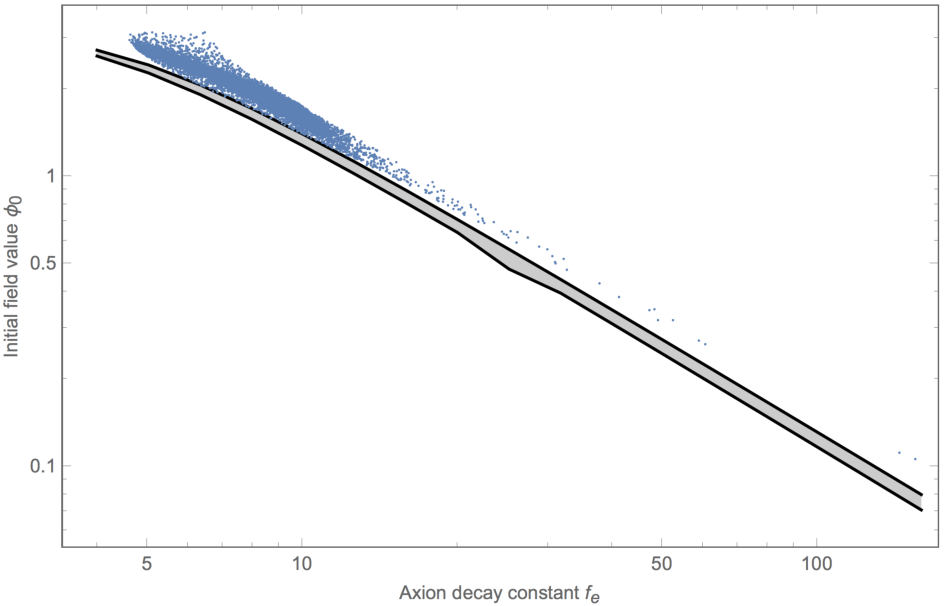
\includegraphics[width=0.5\textwidth]{figs/figc.pdf}
  \caption{Comparison of parameter region $\left({\phi}_{0}, f\right)$ for points from Fig.(\ref{Figure:fig.enhancement.sim}) (blue) vs. the corresponding parameter region for true Natural Inflation (gray). In both cases the pivot number of e-foldings is between $50$ and $60$. The systematic shift may be specific to considered DBI model.}
  \label{fig.comparison.sim}
\end{figure}


\begin{thebibliography}{99}

  %\cite{Guth:1980zm}
  \bibitem{Guth:1980zm}
  A.~H.~Guth,
  %``The Inflationary Universe: A Possible Solution to the Horizon and Flatness Problems,''
  Phys.\ Rev.\ D {\bf 23}, 347 (1981)
  [Adv.\ Ser.\ Astrophys.\ Cosmol.\ {\bf 3}, 139 (1987)].
  doi:10.1103/PhysRevD.23.347
  %%CITATION = doi:10.1103/PhysRevD.23.347;%%
  %7212 citations counted in INSPIRE as of 01 Apr 2019


  %\cite{Starobinsky:1980te}
  \bibitem{Starobinsky:1980te}
  A.~A.~Starobinsky,
  %``A New Type of Isotropic Cosmological Models Without Singularity,''
  Phys.\ Lett.\ B {\bf 91}, 99 (1980)
  [Phys.\ Lett.\ {\bf 91B}, 99 (1980)]
  [Adv.\ Ser.\ Astrophys.\ Cosmol.\ {\bf 3}, 130 (1987)].
  doi:10.1016/0370-2693(80)90670-X
  %%CITATION = doi:10.1016/0370-2693(80)90670-X;%%
  %4010 citations counted in INSPIRE as of 01 Apr 2019


  %\cite{Linde:1981mu}
  \bibitem{Linde:1981mu}
  A.~D.~Linde,
  %``A New Inflationary Universe Scenario: A Possible Solution of the Horizon, Flatness, Homogeneity, Isotropy and Primordial Monopole Problems,''
  Phys.\ Lett.\ {\bf 108B}, 389 (1982)
  [Adv.\ Ser.\ Astrophys.\ Cosmol.\ {\bf 3}, 149 (1987)].
  doi:10.1016/0370-2693(82)91219-9
  %%CITATION = doi:10.1016/0370-2693(82)91219-9;%%
  %4484 citations counted in INSPIRE as of 01 Apr 2019


  %\cite{Albrecht:1982wi}
  \bibitem{Albrecht:1982wi}
  A.~Albrecht and P.~J.~Steinhardt,
  %``Cosmology for Grand Unified Theories with Radiatively Induced Symmetry Breaking,''
  Phys.\ Rev.\ Lett.\ {\bf 48}, 1220 (1982)
  [Adv.\ Ser.\ Astrophys.\ Cosmol.\ {\bf 3}, 158 (1987)].
  doi:10.1103/PhysRevLett.48.1220
  %%CITATION = doi:10.1103/PhysRevLett.48.1220;%%
  %3920 citations counted in INSPIRE as of 01 Apr 2019


  \bibitem{Sato}
  K.~Sato,
  Monthly Notices of the Royal Astronomical Society, Volume 195, Issue 3, 1 July 1981, Pages 467-479,https://doi.org/10.1093/mnras/195.3.467




  %\cite{Linde:1983gd}
  \bibitem{Linde:1983gd}
  A.~D.~Linde,
  %``Chaotic Inflation,''
  Phys.\ Lett.\ {\bf 129B}, 177 (1983).
  doi:10.1016/0370-2693(83)90837-7
  %%CITATION = doi:10.1016/0370-2693(83)90837-7;%%
  %2728 citations counted in INSPIRE as of 01 Apr 2019



  \bibitem{Mukhanov+}
  V. F. Mukhanov and G. V. Chibisov, Pis'ma Zh. Eksp. Teor. Fiz. 33, 549 (1981) [JETP Lett. 33, 532 (1981)]; S. W. Hawking, Phys. Lett. B 115, 295 (1982); A. A. Starobinsky, Phys. Lett. B 117, 175 (1982); A. H. Guth and S. Y. Pi, Phys. Rev. Lett. 49, 1110 (1982); J. M. Bardeen, P. J. Steinhardt, and M. S. Turner, Phys. Rev. D 28, 679 (1983).



  %\cite{Cheung:2007st}
  \bibitem{Cheung:2007st}
  C.~Cheung, P.~Creminelli, A.~L.~Fitzpatrick, J.~Kaplan and L.~Senatore,
  %``The Effective Field Theory of Inflation,''
  JHEP {\bf 0803}, 014 (2008)
  doi:10.1088/1126-6708/2008/03/014
  [arXiv:0709.0293 [hep-th]].
  %%CITATION = doi:10.1088/1126-6708/2008/03/014;%%
  %661 citations counted in INSPIRE as of 01 Apr 2019


  %\cite{Adam:2015rua}
  \bibitem{Adam:2015rua}
  R.~Adam {\it et al.} [Planck Collaboration],
  %``Planck 2015 results. I. Overview of products and scientific results,''
  Astron.\ Astrophys.\ {\bf 594}, A1 (2016)
  doi:10.1051/0004-6361/201527101
  [arXiv:1502.01582 [astro-ph.CO]].
  %%CITATION = doi:10.1051/0004-6361/201527101;%%
  %727 citations counted in INSPIRE as of 01 Apr 2019


  %\cite{Ade:2015lrj}
  \bibitem{Ade:2015lrj}
  P.~A.~R.~Ade {\it et al.} [Planck Collaboration],
  %``Planck 2015 results. XX. Constraints on inflation,''
  Astron.\ Astrophys.\ {\bf 594}, A20 (2016)
  doi:10.1051/0004-6361/201525898
  [arXiv:1502.02114 [astro-ph.CO]].
  %%CITATION = doi:10.1051/0004-6361/201525898;%%
  %1912 citations counted in INSPIRE as of 01 Apr 2019


  %\cite{Array:2015xqh}
  \bibitem{Array:2015xqh}
  P.~A.~R.~Ade {\it et al.} [BICEP2 and Keck Array Collaborations],
  %``Improved Constraints on Cosmology and Foregrounds from BICEP2 and Keck Array Cosmic Microwave Background Data with Inclusion of 95 GHz Band,''
  Phys.\ Rev.\ Lett.\ {\bf 116}, 031302 (2016)
  doi:10.1103/PhysRevLett.116.031302
  [arXiv:1510.09217 [astro-ph.CO]].
  %%CITATION = doi:10.1103/PhysRevLett.116.031302;%%
  %492 citations counted in INSPIRE as of 01 Apr 2019


  %\cite{Freese:1990rb}
  \bibitem{Freese:1990rb}
  K.~Freese, J.~A.~Frieman and A.~V.~Olinto,
  %``Natural inflation with pseudo - Nambu-Goldstone bosons,''
  Phys.\ Rev.\ Lett.\ {\bf 65}, 3233 (1990).
  doi:10.1103/PhysRevLett.65.3233
  %%CITATION = doi:10.1103/PhysRevLett.65.3233;%%
  %926 citations counted in INSPIRE as of 01 Apr 2019


  %\cite{Adams:1992bn}
  \bibitem{Adams:1992bn}
  F.~C.~Adams, J.~R.~Bond, K.~Freese, J.~A.~Frieman and A.~V.~Olinto,
  %``Natural inflation: Particle physics models, power law spectra for large scale structure, and constraints from COBE,''
  Phys.\ Rev.\ D {\bf 47}, 426 (1993)
  doi:10.1103/PhysRevD.47.426
  [hep-ph/9207245].
  %%CITATION = doi:10.1103/PhysRevD.47.426;%%
  %515 citations counted in INSPIRE as of 01 Apr 2019


  %\cite{Banks:2003sx}
  \bibitem{Banks:2003sx}
  T.~Banks, M.~Dine, P.~J.~Fox and E.~Gorbatov,
  %``On the possibility of large axion decay constants,''
  JCAP {\bf 0306}, 001 (2003)
  doi:10.1088/1475-7516/2003/06/001
  [hep-th/0303252].
  %%CITATION = doi:10.1088/1475-7516/2003/06/001;%%
  %265 citations counted in INSPIRE as of 01 Apr 2019


  %\cite{Svrcek:2006yi}
  \bibitem{Svrcek:2006yi}
  P.~Svrcek and E.~Witten,
  %``Axions In String Theory,''
  JHEP {\bf 0606}, 051 (2006)
  doi:10.1088/1126-6708/2006/06/051
  [hep-th/0605206].
  %%CITATION = doi:10.1088/1126-6708/2006/06/051;%%
  %641 citations counted in INSPIRE as of 01 Apr 2019


  %\cite{Kim:2004rp}
  \bibitem{Kim:2004rp}
  J.~E.~Kim, H.~P.~Nilles and M.~Peloso,
  %``Completing natural inflation,''
  JCAP {\bf 0501}, 005 (2005)
  doi:10.1088/1475-7516/2005/01/005
  [hep-ph/0409138].
  %%CITATION = doi:10.1088/1475-7516/2005/01/005;%%
  %370 citations counted in INSPIRE as of 01 Apr 2019


  %\cite{Long:2014dta}
  \bibitem{Long:2014dta}
  C.~Long, L.~McAllister and P.~McGuirk,
  %``Aligned Natural Inflation in String Theory,''
  Phys.\ Rev.\ D {\bf 90}, 023501 (2014)
  doi:10.1103/PhysRevD.90.023501
  [arXiv:1404.7852 [hep-th]].
  %%CITATION = doi:10.1103/PhysRevD.90.023501;%%
  %84 citations counted in INSPIRE as of 01 Apr 2019


  %\cite{Nath:2017ihp}
  \bibitem{Nath:2017ihp}
  P.~Nath and M.~Piskunov,
  %``Evidence for Inflation in an Axion Landscape,''
  JHEP {\bf 1803}, 121 (2018)
  doi:10.1007/JHEP03(2018)121
  [arXiv:1712.01357 [hep-ph]].
  %%CITATION = doi:10.1007/JHEP03(2018)121;%%
  %2 citations counted in INSPIRE as of 01 Apr 2019


  %\cite{Nath:2016qzm}
  \bibitem{Nath:2016qzm}
  P.~Nath,
  %``Supersymmetry, Supergravity, and Unification,''
  doi:10.1017/9781139048118
  %%CITATION = doi:10.1017/9781139048118;%%
  %5 citations counted in INSPIRE as of 01 Apr 2019


  %\cite{BlancoPillado:2006he}
  \bibitem{BlancoPillado:2006he}
  J.~J.~Blanco-Pillado, C.~P.~Burgess, J.~M.~Cline, C.~Escoda, M.~Gomez-Reino, R.~Kallosh, A.~D.~Linde and F.~Quevedo,
  %``Inflating in a better racetrack,''
  JHEP {\bf 0609}, 002 (2006)
  doi:10.1088/1126-6708/2006/09/002
  [hep-th/0603129].
  %%CITATION = doi:10.1088/1126-6708/2006/09/002;%%
  %137 citations counted in INSPIRE as of 01 Apr 2019


  %\cite{Conlon:2005jm}
  \bibitem{Conlon:2005jm}
  J.~P.~Conlon and F.~Quevedo,
  %``Kahler moduli inflation,''
  JHEP {\bf 0601}, 146 (2006)
  doi:10.1088/1126-6708/2006/01/146
  [hep-th/0509012].
  %%CITATION = doi:10.1088/1126-6708/2006/01/146;%%
  %229 citations counted in INSPIRE as of 01 Apr 2019


  %\cite{Ben-Dayan:2014lca}
  \bibitem{Ben-Dayan:2014lca}
  I.~Ben-Dayan, F.~G.~Pedro and A.~Westphal,
  %``Towards Natural Inflation in String Theory,''
  Phys.\ Rev.\ D {\bf 92}, no. 2, 023515 (2015)
  doi:10.1103/PhysRevD.92.023515
  [arXiv:1407.2562 [hep-th]].
  %%CITATION = doi:10.1103/PhysRevD.92.023515;%%
  %50 citations counted in INSPIRE as of 01 Apr 2019


  %\cite{Gao:2014uha}
  \bibitem{Gao:2014uha}
  X.~Gao, T.~Li and P.~Shukla,
  %``Combining Universal and Odd RR Axions for Aligned Natural Inflation,''
  JCAP {\bf 1410}, 048 (2014)
  doi:10.1088/1475-7516/2014/10/048
  [arXiv:1406.0341 [hep-th]].
  %%CITATION = doi:10.1088/1475-7516/2014/10/048;%%
  %42 citations counted in INSPIRE as of 01 Apr 2019


  %\cite{Kallosh:1995hi}
  \bibitem{Kallosh:1995hi}
  R.~Kallosh, A.~D.~Linde, D.~A.~Linde and L.~Susskind,
  %``Gravity and global symmetries,''
  Phys.\ Rev.\ D {\bf 52}, 912 (1995)
  doi:10.1103/PhysRevD.52.912
  [hep-th/9502069].
  %%CITATION = doi:10.1103/PhysRevD.52.912;%%
  %303 citations counted in INSPIRE as of 01 Apr 2019


  %\cite{Chamseddine:1982jx}
  \bibitem{Chamseddine:1982jx}
  A.~H.~Chamseddine, R.~L.~Arnowitt and P.~Nath,
  %``Locally Supersymmetric Grand Unification,''
  Phys.\ Rev.\ Lett.\ {\bf 49}, 970 (1982).
  doi:10.1103/PhysRevLett.49.970
  %%CITATION = doi:10.1103/PhysRevLett.49.970;%%
  %1991 citations counted in INSPIRE as of 01 Apr 2019


  %\cite{Cremmer:1982en}
  \bibitem{Cremmer:1982en}
  E.~Cremmer, S.~Ferrara, L.~Girardello and A.~Van Proeyen,
  %``Yang-Mills Theories with Local Supersymmetry: Lagrangian, Transformation Laws and SuperHiggs Effect,''
  Nucl.\ Phys.\ B {\bf 212}, 413 (1983).
  doi:10.1016/0550-3213(83)90679-X
  %%CITATION = doi:10.1016/0550-3213(83)90679-X;%%
  %1189 citations counted in INSPIRE as of 01 Apr 2019


  %\cite{Nath:1983aw}
  \bibitem{Nath:1983aw}
  P.~Nath, R.~L.~Arnowitt and A.~H.~Chamseddine,
  %``Gauge Hierarchy in Supergravity Guts,''
  Nucl.\ Phys.\ B {\bf 227}, 121 (1983).
  doi:10.1016/0550-3213(83)90145-1
  %%CITATION = doi:10.1016/0550-3213(83)90145-1;%%
  %309 citations counted in INSPIRE as of 01 Apr 2019


  %\cite{Kachru:2003aw}
  \bibitem{Kachru:2003aw}
  S.~Kachru, R.~Kallosh, A.~D.~Linde and S.~P.~Trivedi,
  %``De Sitter vacua in string theory,''
  Phys.\ Rev.\ D {\bf 68}, 046005 (2003)
  doi:10.1103/PhysRevD.68.046005
  [hep-th/0301240].
  %%CITATION = doi:10.1103/PhysRevD.68.046005;%%
  %2667 citations counted in INSPIRE as of 01 Apr 2019


  %\cite{Balasubramanian:2005zx}
  \bibitem{Balasubramanian:2005zx}
  V.~Balasubramanian, P.~Berglund, J.~P.~Conlon and F.~Quevedo,
  %``Systematics of moduli stabilisation in Calabi-Yau flux compactifications,''
  JHEP {\bf 0503}, 007 (2005)
  doi:10.1088/1126-6708/2005/03/007
  [hep-th/0502058].
  %%CITATION = doi:10.1088/1126-6708/2005/03/007;%%
  %735 citations counted in INSPIRE as of 01 Apr 2019


  %\cite{Khoury:2010gb}
  \bibitem{Khoury:2010gb}
  J.~Khoury, J.~L.~Lehners and B.~Ovrut,
  %``Supersymmetric P(X,$\phi$) and the Ghost Condensate,''
  Phys.\ Rev.\ D {\bf 83}, 125031 (2011)
  doi:10.1103/PhysRevD.83.125031
  [arXiv:1012.3748 [hep-th]].
  %%CITATION = doi:10.1103/PhysRevD.83.125031;%%
  %87 citations counted in INSPIRE as of 01 Apr 2019


  %\cite{Khoury:2011da}
  \bibitem{Khoury:2011da}
  J.~Khoury, J.~L.~Lehners and B.~A.~Ovrut,
  %``Supersymmetric Galileons,''
  Phys.\ Rev.\ D {\bf 84}, 043521 (2011)
  doi:10.1103/PhysRevD.84.043521
  [arXiv:1103.0003 [hep-th]].
  %%CITATION = doi:10.1103/PhysRevD.84.043521;%%
  %91 citations counted in INSPIRE as of 01 Apr 2019


  %\cite{Baumann:2011nk}
  \bibitem{Baumann:2011nk}
  D.~Baumann and D.~Green,
  %``Signatures of Supersymmetry from the Early Universe,''
  Phys.\ Rev.\ D {\bf 85}, 103520 (2012)
  doi:10.1103/PhysRevD.85.103520
  [arXiv:1109.0292 [hep-th]].
  %%CITATION = doi:10.1103/PhysRevD.85.103520;%%
  %164 citations counted in INSPIRE as of 01 Apr 2019


  %\cite{Baumann:2011nm}
  \bibitem{Baumann:2011nm}
  D.~Baumann and D.~Green,
  %``Supergravity for Effective Theories,''
  JHEP {\bf 1203}, 001 (2012)
  doi:10.1007/JHEP03(2012)001
  [arXiv:1109.0293 [hep-th]].
  %%CITATION = doi:10.1007/JHEP03(2012)001;%%
  %36 citations counted in INSPIRE as of 01 Apr 2019


  %\cite{Rocek:1997hi}
  \bibitem{Rocek:1997hi}
  M.~Rocek and A.~A.~Tseytlin,
  %``Partial breaking of global D = 4 supersymmetry, constrained superfields, and three-brane actions,''
  Phys.\ Rev.\ D {\bf 59}, 106001 (1999)
  doi:10.1103/PhysRevD.59.106001
  [hep-th/9811232].
  %%CITATION = doi:10.1103/PhysRevD.59.106001;%%
  %191 citations counted in INSPIRE as of 01 Apr 2019


  %\cite{Tseytlin:1999dj}
  \bibitem{Tseytlin:1999dj}
  A.~A.~Tseytlin,
  %``Born-Infeld action, supersymmetry and string theory,''
  In *Shifman, M.A. (ed.): The many faces of the superworld* 417-452
  % doi:10.1142/9789812793850_0025
  [hep-th/9908105].
  %%CITATION = doi:10.1142/9789812793850_0025;%%
  %411 citations counted in INSPIRE as of 01 Apr 2019


  %\cite{Ito:2007hy}
  \bibitem{Ito:2007hy}
  K.~Ito, H.~Nakajima and S.~Sasaki,
  %``Deformation of super Yang-Mills theories in R-R 3-form background,''
  JHEP {\bf 0707}, 068 (2007)
  doi:10.1088/1126-6708/2007/07/068
  [arXiv:0705.3532 [hep-th]].
  %%CITATION = doi:10.1088/1126-6708/2007/07/068;%%
  %13 citations counted in INSPIRE as of 01 Apr 2019


  %\cite{Billo:2008sp}
  \bibitem{Billo:2008sp}
  M.~Billo, L.~Ferro, M.~Frau, F.~Fucito, A.~Lerda and J.~F.~Morales,
  %``Flux interactions on D-branes and instantons,''
  JHEP {\bf 0810}, 112 (2008)
  doi:10.1088/1126-6708/2008/10/112
  [arXiv:0807.1666 [hep-th]].
  %%CITATION = doi:10.1088/1126-6708/2008/10/112;%%
  %54 citations counted in INSPIRE as of 01 Apr 2019


  %\cite{Sasaki:2012ka}
  \bibitem{Sasaki:2012ka}
  S.~Sasaki, M.~Yamaguchi and D.~Yokoyama,
  %``Supersymmetric DBI inflation,''
  Phys.\ Lett.\ B {\bf 718}, 1 (2012)
  doi:10.1016/j.physletb.2012.10.006
  [arXiv:1205.1353 [hep-th]].
  %%CITATION = doi:10.1016/j.physletb.2012.10.006;%%
  %34 citations counted in INSPIRE as of 01 Apr 2019


  %\cite{Aoki:2016tod}
  \bibitem{Aoki:2016tod}
  S.~Aoki and Y.~Yamada,
  %``More on DBI action in 4D $ \mathcal{N} $ = 1 supergravity,''
  JHEP {\bf 1701}, 121 (2017)
  doi:10.1007/JHEP01(2017)121
  [arXiv:1611.08426 [hep-th]].
  %%CITATION = doi:10.1007/JHEP01(2017)121;%%
  %3 citations counted in INSPIRE as of 01 Apr 2019


  %\cite{Nath:2018xxe}
  \bibitem{Nath:2018xxe}
  P.~Nath and M.~Piskunov,
  %``Supersymmetric Dirac-Born-Infeld Axionic Inflation and Non-Gaussianity,''
  JHEP {\bf 1902}, 034 (2019)
  doi:10.1007/JHEP02(2019)034
  [arXiv:1807.02549 [hep-ph]].
  %%CITATION = doi:10.1007/JHEP02(2019)034;%%

\end{thebibliography}

\end{document}
